\chapter{Capa de Migración e Implementación}
\section{Introducción}
Esta capa describe la implementación de modelos y características de migración para   ejecutar un cambio en la arquitectura del negocio. Cada uno de los puntos de vista que contiene esta capa presenta una perspectiva  para modelar la gestión del cambio de arquitectura, modelar la transición de una arquitectura existente a una arquitectura de destino y definir las relaciones entre los programas y proyectos y las partes de la arquitectura que implementan \cite{ArchiMate3.0.1}. 

Esta capa da conocer el contexto sobre el cual se busca modelar el cambio estructural de la arquitectura empresarial. Para una adecuada apropiación de la conceptualización de esta capa, se implementa el uso de tres diferentes puntos de vista (proyecto,migración y migración e implementación). En esta capa se retoman algunos de los conceptos utilizados en la capa de negocio como por ejemplo el concepto de objeto de negocio representado en esta capa como un Paquete de Trabajo
(Work Package) y el concepto de representación el cual tiene como
equivalente un Liberable (Derivable)\cite{BolanosCastro2019}.


A continuación se presentan cada uno de los puntos de vista de la capa de Implementación a partir del soporte realizado por el Área de Investigación de Análisis de datos a los investigadores de la Subdirección de Investigaciones, otras Subdirecciones y demás unidades funcionales del Instituto de Cancerología.

%-------------Punto de Vista de Proyecto----------%
\newpage
\section{Punto de Vista de Proyecto}
El punto de vista de proyecto se utiliza principalmente para modelar la gestión del cambio de la arquitectura permitiendo al diseñador o analista plasmar mediante un diagrama el proceso de interacción de los diferentes elementos\cite{BolanosCastro2019}. 

En la Figura \ref{PvProyecto} se plantea el Caso para el Punto de Vista de Proyecto con cada uno de los elementos que interactúan entre sí. 

\begin{figure}[h!]
	\centering
	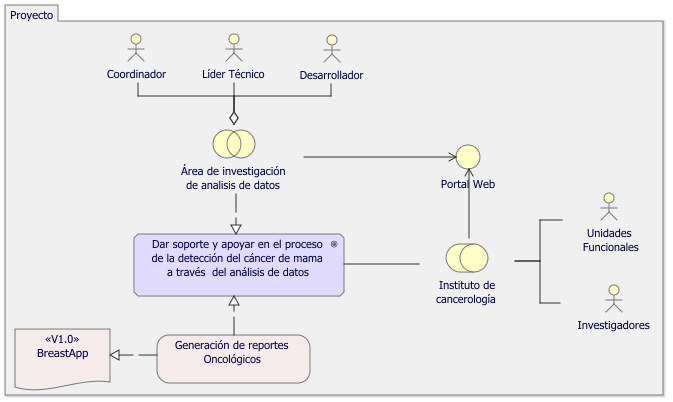
\includegraphics[width=1\linewidth]{ARQUITECTURA/imgs/CapaImplementacion/1_PvProyecto}
	\caption{Punto de Vista de Proyecto}
	\label{PvProyecto}
\end{figure}

\begin{enumerate}[label=\textbf{\arabic*})]

\item  \textbf{\textbf{Instituto  de Cancerología}:} Este elemento hace referencia a el rol de la organización el cual cuenta con siete grupos de investigación que desarrollan diversas actividades según su campo de acción: investigación clínica, investigación epidemológica, biología del cáncer e investigación en el área de la salud pública.A este rol están asociados el actor \textit{Investigador } y el actor \textit{Unidades funcionales }. Estos roles se describen a continuación: 
\newpage
\begin{itemize}
	\item  \textbf{\textit{Investigadores :}}  Este rol está conformado por todos los grupos de investigación en cáncer del país registrados ante Colciencias y adicionalmente, con representantes de diferentes tipos de usuarios del conocimiento generado por la investigación como son las sociedades médicas, los prestadores de servicios oncológicos, los aseguradores, las autoridades sanitarias y los pacientes entre otros. 
	
	\item  \textbf{\textit{Unidades Funcionales :}}  Este rol está conformado por las unidades clínicas ubicadas al interior del Instituto  de Cancerología cuya función es evaluar la situación de salud del paciente con diagnóstico presuntivo de cáncer. 
\end{itemize}

\item \textbf{Área de Investigación de análisis de datos:} Corresponde a una de las dependencias del área de investigación la cual  tiene por objetivo dar soporte a los investigadores de la Subdirección de Investigaciones, otras Subdirecciones y demás unidades funcionales del Instituto  de Cancerología, haciendo uso de métodos computacionales para el manejo y análisis de datos Oncológicos. Este actor tiene \textit{agregado} tres actores los cuales se muestran a continuación:

\begin{itemize}
\item  \textbf{\textit{Coordinador:}}
Es la persona encargada de regular, gestionar, dirigir y supervisar el Área de Investigación de análisis de datos de Oncología para que el soporte realizado a los investigadores de la Subdirección de Investigaciones, otras Subdirecciones y demás unidades funcionales se realice correctamente.
		
\item  \textbf{\textit{Líder Técnico:}}
Es la persona con conocimiento técnico avanzado en los temas de análisis de datos de Oncología y es el  responsable de asignar y definir las  tareas y el tiempo necesario en el desarrollo e implementación de los recursos  según las necesidades presentadas por los investigadores y las unidades funcionales del Instituto  de Cancerología.

\item  \textbf{\textit{Desarrollador:}}
Es la persona encargada de cumplir con las implementaciones presentadas en el ámbito de análisis de datos de Oncología y que da  solución a cada uno de los requerimientos y necesidades presentadas por los  investigadores y las unidades funcionales del Instituto  de Cancerología.
\end{itemize}

\item  \textbf{Portal Web :} Es el medio de comunicación entre el Área de Investigación de análisis de datos  y los investigadores de la Subdirección de Investigaciones, otras Subdirecciones y demás unidades funcionales del Instituto  de Cancerología. Esta interfaz tiene una asociación con el rol del  \textit{Área de Investigación de análisis de datos}  y es usada por el rol \textit{Instituto  de Cancerología}.


\item  \textbf{Dar soporte y apoyar en el proceso de la detección del cáncer de mama a través del análisis de datos:} Este objetivo organizacional hace referencia a el servicio de generar diagnósticos relacionados con el cáncer de mama  solicitados por los diferentes funcionarios del Instituto de Cancerología.

\item  \textbf{Generación de reportes oncológicos:} Es el paquete de trabajo principal del instituto de Cancerología basado en la estrategia planteada y los recursos disponibles identificados. La meta es construir una  aplicación web que genere  informes tipo reporte con base a los resultados arrojados por  diferentes modelos de Machine Learning, en donde se de un resultado definitivo acerca del  padecimiento de Cáncer de mama.Este diagnostico se realiza con el propósito de dar soporte a los investigadores de la Subdirección de Investigaciones, otras Subdirecciones y demás unidades funcionales del Instituto  de Cancerología.

\item  \textbf{BreastApp:} Representa el liberable, consecuencia del paquete de
trabajo definido anteriormente. Este producto corresponde a la generación de reportes diagnósticos según el análisis de datos oncológicos elaborados por los investigadores de la Subdirección de Investigaciones, otras Subdirecciones y demás unidades funcionales del Instituto  de Cancerología.Es el resultado obtenido que cumple con los objetivos planteados y satisface las necesidades de la organización.
\end{enumerate}

%-------------Punto de Vista de Migracion----------%
\newpage
\section{Punto de Vista de Migración}
El Punto de Vista de Migración implica modelos y conceptos que pueden usarse para especificar la transición de una arquitectura existente a una arquitectura deseada.\cite{BolanosCastro2019}. 

En la Figura \ref{PvMigracion} se plantea el Caso para el Punto de Vista de Migración con cada uno de los elementos que interactúan entre sí. 

\begin{figure}[h!]
	\centering
	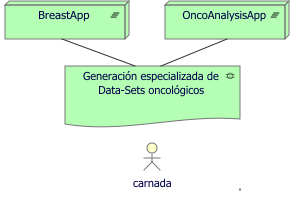
\includegraphics[width=0.75\linewidth]{ARQUITECTURA/imgs/CapaImplementacion/2_PvMigracion}
	\caption{Punto de Vista de Migración}
	\label{PvMigracion}
\end{figure}

\begin{enumerate}[label=\textbf{\arabic*})]
	
\item  \textbf{BreastApp:} Es la Meseta inicial que  corresponde  a una aplicación web la cual genera reportes diagnósticos según el análisis de datos relacionados con el Cáncer de mama elaborados para brindar soporte a los investigadores de la Subdirección de Investigaciones, otras Subdirecciones y demás unidades funcionales del Instituto  de Cancerología.

\item  \textbf{Generación especializada de  Data-Sets oncológicos:} Hace referencia a la brecha que debe resolverse para poder generar la Meseta futura \textit{OncoAnalysisApp}.Esta brecha esta relacionada con la generación dinámica de Data-Sets para cualquier tipo de cáncer.

\item  \textbf{OncoAnalysisApp:} Es la Meseta final de la aplicación. Representa un producto a futuro con nuevas implementaciones y funcionalidades adicionales. En este caso se pretende generar diagnósticos para cualquier tipo de cáncer para brindar un soporte mas amplio a los investigadores de la Subdirección de Investigaciones, otras Subdirecciones y demás unidades funcionales del Instituto  de Cancerología

\end{enumerate}

%-------------Punto de Vista de Migracion----------%
\newpage
\section{Punto de Vista de Migración e implementación}
El Punto de Vista de Migración e Implementación se utiliza para relacionar programas y proyectos con las partes de la arquitectura que implementan\cite{BolanosCastro2019}. 

En la Figura \ref{PvMigraImple} se plantea el Caso para el Punto de Vista de Migración con cada uno de los elementos que interactúan entre sí. 

\begin{figure}[h!]
	\centering
	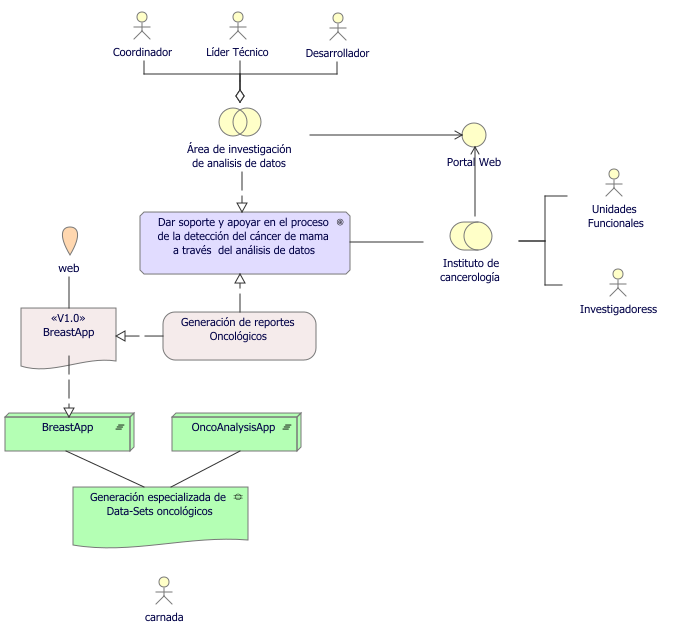
\includegraphics[width=0.92\linewidth]{ARQUITECTURA/imgs/CapaImplementacion/3_PvMigracionImplementacion}
	\caption{Punto de Vista de Migración e Implementación}
	\label{PvMigraImple}
\end{figure}

\begin{enumerate}[label=\textbf{\arabic*})]
	
	\item  \textbf{\textbf{Instituto  de Cancerología}:} Este elemento hace referencia a el rol de la organización el cual cuenta con siete grupos de investigación que desarrollan diversas actividades según su campo de acción: investigación clínica, investigación epidemológica, biología del cáncer e investigación en el área de la salud pública.A este rol están asociados el actor \textit{Investigador } y el actor \textit{Unidades funcionales }. Estos roles se describen a continuación: 
	\begin{itemize}
		\item  \textbf{\textit{Investigadores :}}  Este rol está conformado por todos los grupos de investigación en cáncer del país registrados ante Colciencias y adicionalmente, con representantes de diferentes tipos de usuarios del conocimiento generado por la investigación como son las sociedades médicas, los prestadores de servicios oncológicos, los aseguradores, las autoridades sanitarias y los pacientes entre otros. 
		
		\item  \textbf{\textit{Unidades Funcionales :}}  Este rol está conformado por las unidades clínicas ubicadas al interior del Instituto  de Cancerología cuya función es evaluar la situación de salud del paciente con diagnóstico presuntivo de cáncer. 
	\end{itemize}
	
	\item \textbf{Área de Investigación de análisis de datos:} Corresponde a una de las dependencias del área de investigación la cual  tiene por objetivo dar soporte a los investigadores de la Subdirección de Investigaciones, otras Subdirecciones y demás unidades funcionales del Instituto  de Cancerología, haciendo uso de métodos computacionales para el manejo y análisis de datos Oncológicos. Este actor tiene \textit{agregado} tres actores los cuales se muestran a continuación:
	
	\begin{itemize}
		\item  \textbf{\textit{Coordinador:}}
		Es la persona encargada de regular, gestionar, dirigir y supervisar el Área de Investigación de análisis de datos de Oncología para que el soporte realizado a los investigadores de la Subdirección de Investigaciones, otras Subdirecciones y demás unidades funcionales se realice correctamente.
		
		\item  \textbf{\textit{Líder Técnico:}}
		Es la persona con conocimiento técnico avanzado en los temas de análisis de datos de Oncología y es el  responsable de asignar y definir las  tareas y el tiempo necesario en el desarrollo e implementación de los recursos  según las necesidades presentadas por los investigadores y las unidades funcionales del Instituto  de Cancerología.
		
		\item  \textbf{\textit{Desarrollador:}}
		Es la persona encargada de cumplir con las implementaciones presentadas en el ámbito de análisis de datos de Oncología y que da  solución a cada uno de los requerimientos y necesidades presentadas por los  investigadores y las unidades funcionales del Instituto  de Cancerología.
	\end{itemize}
	
	\item  \textbf{Portal Web :} Es el medio de comunicación entre el Área de Investigación de análisis de datos  y los investigadores de la Subdirección de Investigaciones, otras Subdirecciones y demás unidades funcionales del Instituto  de Cancerología. Esta interfaz tiene una asociación con el rol del  \textit{Área de Investigación de análisis de datos}  y es usada por el rol \textit{Instituto  de Cancerología}.
	
	
	\item  \textbf{Dar soporte y apoyar en el proceso de la detección del cáncer de mama a través del análisis de datos:} Este objetivo organizacional hace referencia a el servicio de generar diagnósticos relacionados con el cáncer de mama  solicitados por los diferentes funcionarios del Instituto de Cancerología.
	
	\item  \textbf{Generación de reportes oncológicos:} Es el paquete de trabajo principal del instituto de Cancerología basado en la estrategia planteada y los recursos disponibles identificados. La meta es construir una  aplicación web que genere  informes tipo reporte con base a los resultados arrojados por  diferentes modelos de Machine Learning, en donde se de un resultado definitivo acerca del  padecimiento de Cáncer de mama.Este diagnostico se realiza con el propósito de dar soporte a los investigadores de la Subdirección de Investigaciones, otras Subdirecciones y demás unidades funcionales del Instituto  de Cancerología.
	
	\item  \textbf{BreastApp:} Representa el liberable, consecuencia del paquete de trabajo definido anteriormente. Este producto corresponde a la generación de reportes diagnósticos según el análisis de datos oncológicos elaborados por los investigadores de la Subdirección de Investigaciones, otras Subdirecciones y demás unidades funcionales del Instituto  de Cancerología.Es el resultado obtenido que cumple con los objetivos planteados y satisface las necesidades de la organización. Realiza a la Meseta inicial \textit{BreastApp}
	
	\item  \textbf{Generación especializada de  Data-Sets oncológicos:} Hace referencia a la brecha que debe resolverse para poder generar la Meseta futura \textit{OncoAnalysisApp}.Esta brecha esta relacionada con la generación dinámica de Data-Sets para cualquier tipo de cáncer.
	
	\item  \textbf{OncoAnalysisApp:} Es la Meseta final de la aplicación. Representa un producto a futuro con nuevas implementaciones y funcionalidades adicionales. En este caso se pretende generar diagnósticos para cualquier tipo de cáncer para brindar un soporte mas amplio a los investigadores de la Subdirección de Investigaciones, otras Subdirecciones y demás unidades funcionales del Instituto  de Cancerología
	
	\item  \textbf{Web:} Hace referencia a la ubicación en donde los investigadores de la Subdirección de Investigaciones, otras Subdirecciones y demás unidades funcionales del Instituto de Cancerología pueden acceder a la aplicación \textit{BreastApp}.
\end{enumerate}


